\documentclass[a4paper 10pt]{article}
\usepackage[english,polish]{babel}
\usepackage[MeX]{polski}
\usepackage[utf8]{inputenc}
\usepackage[T1]{fontenc}
\usepackage[letterpaper, portrait, margin=0.5in]{geometry}
\usepackage{graphicx}
\usepackage{listings}
\usepackage{subfigure}
\usepackage{dashrule}
\usepackage{listings}
\usepackage{float}
\usepackage{amsmath}
\usepackage{listings}
\usepackage{multirow}
\usepackage{amsmath}
\usepackage{xcolor}
\usepackage{listings}
\usepackage{hyperref}
\hypersetup{ hidelinks = true, } 
\lstset{
    frame=single,
    breaklines=true,
    postbreak=\raisebox{0ex}[0ex][0ex]{\ensuremath{\color{red}\hookrightarrow\space}}
}


\renewcommand{\rmdefault}{ptm}
  
\frenchspacing

% Used to add additional dot in enumerations
\usepackage{titlesec}
\titlelabel{\thetitle.\quad}
\title{\textbf{Techniki Optymalizacji} \\
Laboratorium nr 4 \\
Sprawozdanie}
\author{Paulina Sadowska, Rafał Araszkiewicz}
\begin{document}
\maketitle

\section{Wprowadzenie}
Celem ćwiczenia było wyznaczenie średniego podobieństwa pomiędzy trasami wyznaczonymi za pomocą algorytmu losowego z Local Search, następnie przedstawienie obliczonych wartości na wykresie i wyznaczenie korelacji. Kolejnym zadaniem było porównanie tras z najlepszą z nich, przedstawienie wyników i również obliczenie współczynnika korelacji.

\section{Otrzymane wyniki}

\begin{figure} [H]
\centering
\caption{Średnie podobieństwo wierzchołkowe do pozostałych rozwiązań (\textbf{współczynnik korelacji = -0,36})}
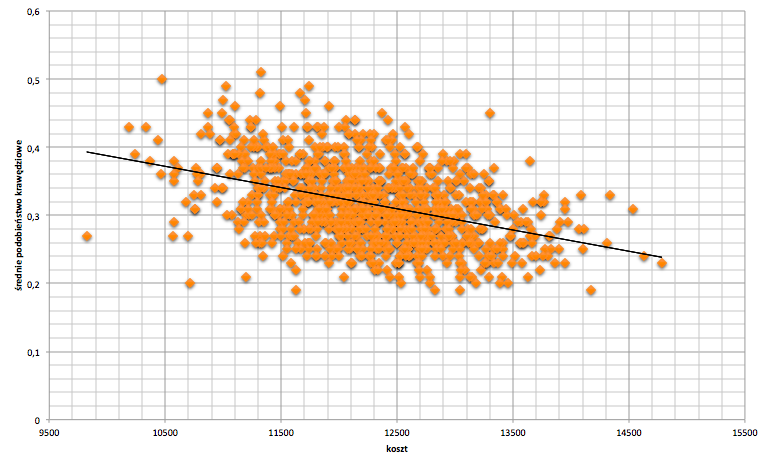
\includegraphics[angle=0,width = 1\textwidth, height=!]{images/edge.png}
\label{Rys. Edges}
\end{figure}

\begin{figure} [H]
\centering
\caption{Średnie podobieństwo krawędzi do pozostałych rozwiązań (\textbf{współczynnik korelacji = -0,65})}
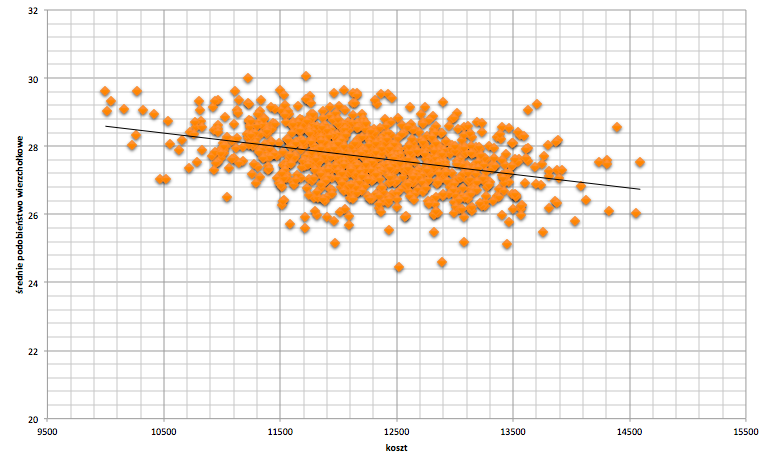
\includegraphics[angle=0,width = 1\textwidth, height=!]{images/node.png}
\label{Rys. Node}
\end{figure}

\begin{figure} [H]
\centering
\caption{Podobieństwo wierzchołkowe do najlepszego z rozwiązań (\textbf{współczynnik korelacji = 0,37})}
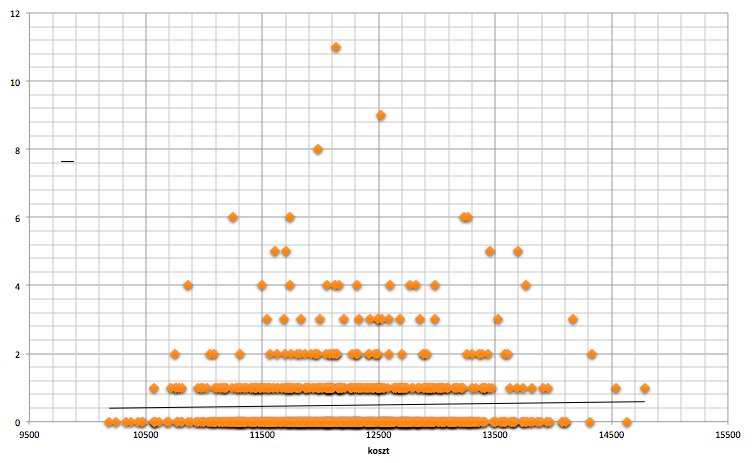
\includegraphics[angle=0,width = 1\textwidth, height=!]{images/node_best.png}
\label{Rys. Edges}
\end{figure}

\begin{figure} [H]
\centering
\caption{Podobieństwo krawędzi do najlepszego z rozwiązań (\textbf{współczynnik korelacji = 0,11})}
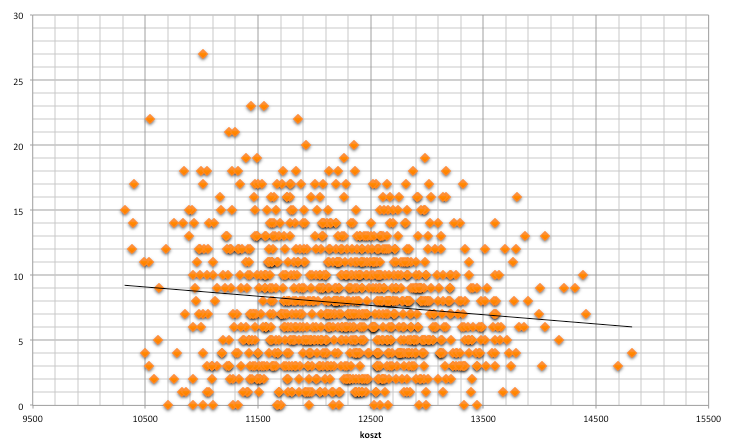
\includegraphics[angle=0,width = 1\textwidth, height=!]{images/edge_best.png}
\label{Rys. Edges}
\end{figure}
\end{document}
\\